%-------------------------------------------------------------------------------
%                                PREAMBLE
%-------------------------------------------------------------------------------
\documentclass[usenames,dvipsnames,svgnames,10pt,aspectratio=169]{beamer}
%
\usefonttheme{professionalfonts}
% This theme uses TIKZ: compile twice with PDFLaTeX or LuaLaTeX.
%
%  Options:
%  - [clean]:    clean slides, i.e. logos and footbar are removed
%  - [kth]:      footbar style inspierd to the official KTH template
%  - [nicewave]: a different style of wave is used (not approved by FLOW)
%
\usetheme[clean]{flow}

\usepackage{tikz}
\usetikzlibrary{arrows}
\usetikzlibrary{shapes.geometric, math, positioning, calc, patterns, angles, quotes}
\usetikzlibrary{patterns.meta,decorations.pathmorphing}

\newcommand{\semaphore}[3]{% #1: color of circle,
                           % #2: color of semicircle
                           % #3: angle of semicircle 
  \tikz[node distance=0mm,baseline]
       {
         \node (s1) [circle, fill=#1, minimum size=6mm] {};
         \node      [semicircle, fill=#2, 
           inner sep=0pt, outer sep=0pt, minimum size=3mm,
           anchor=south,
           at={(s1.center)}, rotate=#3] {};
       }
}

\usepackage[]{circuitikz}

\usepackage{pgfplots}
\usepgfplotslibrary{polar}

\usepackage{hyperref,graphicx,lmodern}
\usepackage[utf8]{inputenc}
\usepackage{media9}
\usepackage{xcolor}
\usepackage{stmaryrd}
\usepackage{nicefrac}
\usepackage{multimedia}
\usepackage{multicol}
\usepackage{upgreek}
\usepackage[]{bm}
\usepackage[]{url}
\usepackage[]{animate}
\usepackage{amsmath}

\graphicspath{{imgs/}}
\setbeamertemplate{blocks}[rounded][shadow=true]

\DeclareMathOperator*{\maximize}{maximize~}

%-------------------------------------------------------------------------------
%                                TITLE PAGE
%-------------------------------------------------------------------------------
\title[Nonlinear physics] % Short title used in footline
{
	Limit cycles are all you have
}

\author[J.-Ch.~Loiseau] % Presenting author in short form used in footline
{
	\underline{Jean-Christophe Loiseau}
}
% - Give the names in the same order as the appear in the paper.
% - Underline the presenting author.

\institute[unused]
{
	\url{jean-christophe.loiseau@ensam.eu} \\
	Laboratoire DynFluid \\
	Arts et M\'etiers, France.
}
% Keep it simple, no one is interested in your street address.

% University logo(s)
\logot{
\includegraphics[width=.128\paperwidth]{DynFluid_logo}}  % Top logo
\logob{
\includegraphics[width=0.128\paperwidth]{ENSAM_logo}} % Bottom logo
% \logoc[{\includegraphics[width=.128\paperwidth]{limsi}}]{\includegraphics[width=.128\paperwidth]{limsi}} % Corner logo
%
% Cover image: \cvrimg{x position}{y position}{cover image}
\cvrimg{.77}{.8}{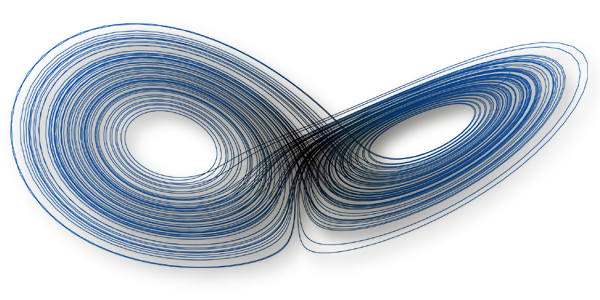
\includegraphics[width=.4\paperwidth]{cover.png}}

\date[unused]{Physique non-lin\'eaire -- 2019-2020}

\begin{document}

\titleframe	% Print the title as the first slide

%-------------------------------------------------------------------------------
%                           PRESENTATION SLIDES
%-------------------------------------------------------------------------------

\begin{frame}[t, c]{Poincaré-Bendixson theorem}{}
  \begin{minipage}{.48\textwidth}
    \centering
    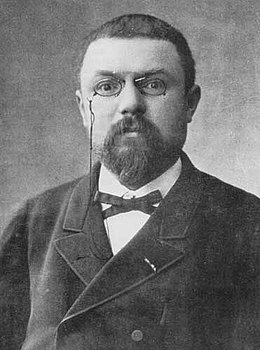
\includegraphics[height=.5\textheight]{poincare}

    \bigskip

    \small
    Henri Poincaré (1854-1912)
  \end{minipage}%
  \hfill
  \begin{minipage}{.48\textwidth}
    \centering
    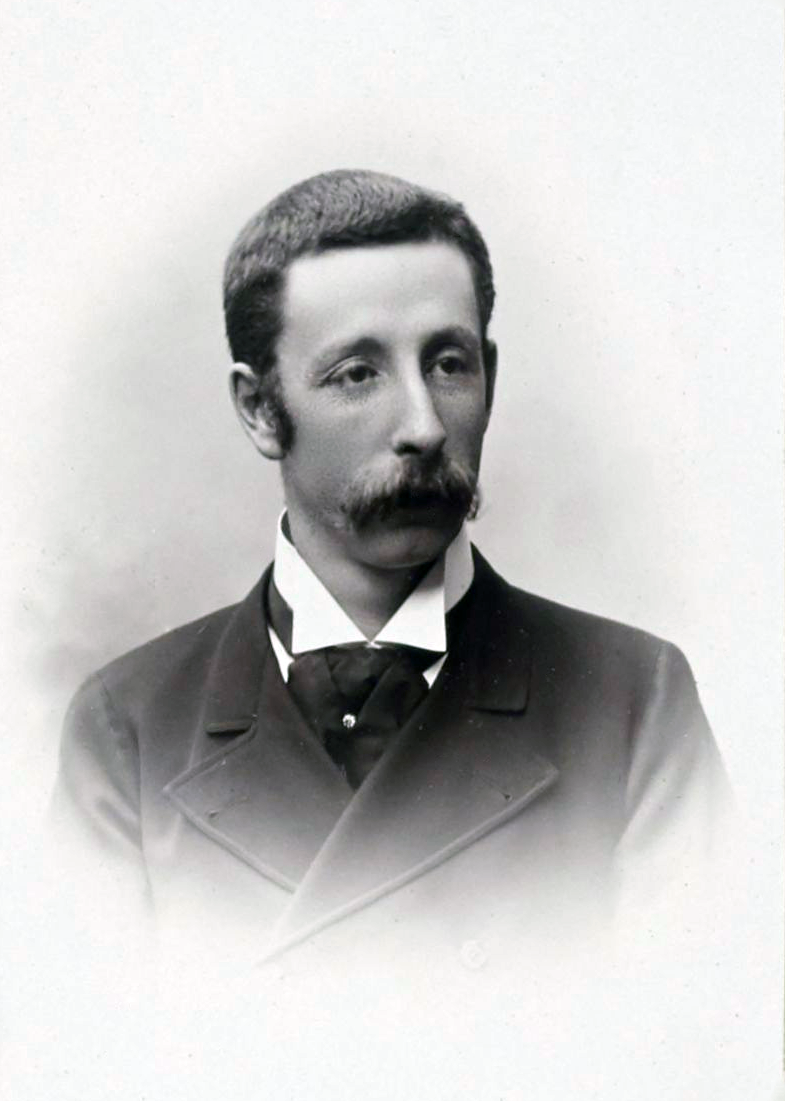
\includegraphics[height=.5\textheight]{bendixson}

    \bigskip

    \small
    Ivar Otto Bendixson (1861-1935)
  \end{minipage}
\end{frame}

\begin{frame}[t, c]{Poincaré-Bendixson theorem}{}
  \begin{minipage}{.68\textwidth}
    \textbf{Poincaré-Bendixson theorem:} Let us suppose that
    %
    \begin{enumerate}
    \item $R$ is a closed, bounded subset of the plane.
    \item $\dot{\bm{x}} = f(\bm{x})$ is a continuously differentiable vector field on an open set containing $R$.
    \item $R$ does not contain any fixed points.
    \item There exists a trajectory $C$ ``confined'' in $R$ (i.e. it starts in $R$ and stays in $R$ for all times).
    \end{enumerate}
    %
    Then, either $C$ is a closed orbit or it spirals toward a closed orbit as $t \to \infty$.
    In either case, $R$ \emph{contains a closed orbit}!
  \end{minipage}%
  \hfill
  \begin{minipage}{.28\textwidth}
    \centering
    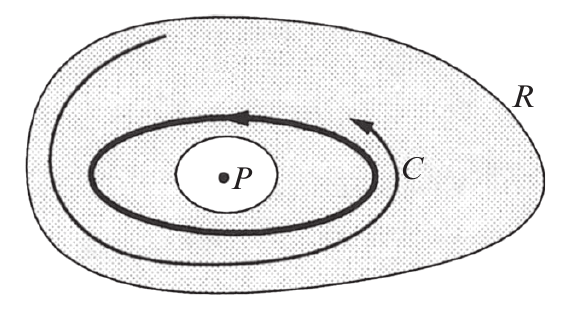
\includegraphics[width=\textwidth]{pb_theorem}
  \end{minipage}
\end{frame}

\begin{frame}[t, c]{A predator-prey model}{}
  \begin{minipage}{.68\textwidth}
    Consider the following predator-prey model
    %
    \[
    \begin{aligned}
      \dot{x} & = g(x)x - p(x)y \\
      \dot{y} & = \left( q(x) - d \right)y,
    \end{aligned}
    \]
    %
    with $d > 0$, while $x(t)$ and $y(t)$ are the prey and predator densities.
  \end{minipage}%
  \hfill
  \begin{minipage}{.28\textwidth}
    \centering
    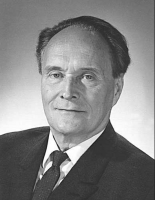
\includegraphics[width=.8\textwidth]{gause}

    \bigskip
    \small
    Georgii Frantsevich Gause (1910-1986)
  \end{minipage}
\end{frame}

\begin{frame}[t, c]{A predator-prey model}{}
  \[
  \begin{aligned}
    \dot{x} & = g(x) x - p(x) y \\
    \dot{y} & = \left( q(x) - d \right) y
  \end{aligned}
  \]
\end{frame}

\begin{frame}[t, c]{A predator-prey model}{}
  \begin{minipage}{.68\textwidth}
    The function $g(x)$ describes the evolution of the prey population in the absence of predation.
    Self-regulation in the prey implies there exists a $K > 0$ so that

    \begin{itemize}
    \item $g(x) > 0$ for $x < K$,
    \item $g(K) = 0$,
    \item $g(x) < 0$ for $x > K$.
    \end{itemize}

    \medskip

    The constant $K$ is known as the \alert{\textbf{prey carrying capacity}}.
  \end{minipage}%
  \hfill
  \begin{minipage}{.28\textwidth}
  \end{minipage}
\end{frame}

\begin{frame}[t, c]{A predator-prey model}{}
  \begin{minipage}{.68\textwidth}
    The function $p(x)$ is the \alert{\textbf{predator trophic function}}.
    It describes the number of prey killed by one predator.
    Its fundamental properties are

    \begin{itemize}
    \item $p(0) = 0$ and $p(x) > 0$ for all $x \in \mathbb{R}_+$.
    \item Reasonable to assume that $\displaystyle \lim_{x \to +\infty} p(x) = C$.
    \end{itemize}

    \medskip

    Three types of predator trophic functions exist, depending on extra assumptions made about $p(x)$.

  \end{minipage}%
  \hfill
  \begin{minipage}{.28\textwidth}
  \end{minipage}
\end{frame}

\begin{frame}[t, c]{A predator-prey model}{}
  \begin{minipage}{.68\textwidth}
    The function $q(x)$ describes the consumption of prey and conversion into predator individuals.
    It can be independent of $p(x)$ albeit we often have $p(x) = q(x)$ (e.g. Lotka-Volterra).
    We require that $q(0) = 0$ and $q^{\prime}(x) > 0$ for $x > 0$.
  \end{minipage}%
  \hfill
  \begin{minipage}{.28\textwidth}
  \end{minipage}
\end{frame}

\begin{frame}[t, c]{A predator-prey model}{Isoclines}
  \begin{minipage}{.48\textwidth}
    \centering
    \textbf{Prey equation}

    \[
    x = 0, \quad l_1 = \left\{ (x, y): y = \dfrac{xg(x)}{p(x)} \right\}.
    \]
  \end{minipage}%
  \hfill
  \begin{minipage}{.48\textwidth}
    \centering
    \begin{tikzpicture}[>=stealth]
      \draw[->] (0, 0) -- (5, 0) node[below] {$x(t)$};
      \draw[->] (0, 0) -- (0, 5) node[left] {$y(t)$};

      \draw[thick, blue] (0, 0) -- (0, 4) node[] {};
    \end{tikzpicture}
  \end{minipage}
\end{frame}


\begin{frame}[t, c]{A predator-prey model}{Isoclines}
  \begin{minipage}{.48\textwidth}
    \centering
    \textbf{Predator equation}

    \[
    y = 0, \quad l_2 = \left\{ (x, y): x = \hat{x}, q(\hat{x}) = d \right\}.
    \]
  \end{minipage}%
  \hfill
  \begin{minipage}{.48\textwidth}
    \centering
    \begin{tikzpicture}[>=stealth]
      \draw[->] (0, 0) -- (5, 0) node[below] {$x(t)$};
      \draw[->] (0, 0) -- (0, 5) node[left] {$y(t)$};

      \draw[thick, blue] (0, 0) -- (0, 4) node[] {};
      \draw[thick, red] (0, 0) -- (4, 0) node[] {};
    \end{tikzpicture}
  \end{minipage}
\end{frame}

\begin{frame}[t, c]{A predator-prey model}{}
  \centering
  \begin{tikzpicture}[>=stealth]
    \draw[->] (0, 0) -- (5, 0) node[below] {$x(t)$};
    \draw[->] (0, 0) -- (0, 5) node[left] {$y(t)$};

    \node[circle, fill=white, draw=black, inner sep=0pt, minimum size=4pt] (a) at (0, 0) {};

  \end{tikzpicture}
\end{frame}

\begin{frame}[t, c]{Why is this theorem so important?}{}
  \begin{minipage}{.68\textwidth}
    It is one of the central results of nonlinear dynamics.
    Dynamical possibilites in the phase plane are very limited: if a trajectory is confined to a closed bounded region with no fixed points, it must eventually approach a \alert{\textbf{closed orbit}}.
    Nothing more complicated is possible!
  \end{minipage}%
  \hfill
  \begin{minipage}{.28\textwidth}
  \end{minipage}
\end{frame}

\begin{frame}[t, c]{No chaos in phase plane!}{}
  \centering
  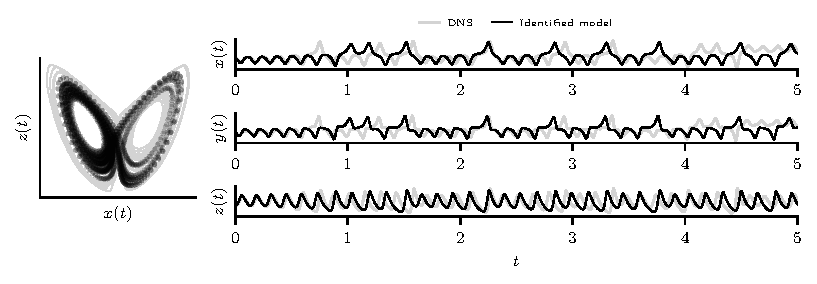
\includegraphics[width=\textwidth]{attractor_comparison_bis}
\end{frame}

\end{document}
